% Paper template for TAR 2016
% (C) 2014 Jan Šnajder, Goran Glavaš, Domagoj Alagić, Mladen Karan
% TakeLab, FER

\documentclass[10pt, a4paper]{article}

\usepackage{tar2016}

\usepackage[utf8]{inputenc}
\usepackage[pdftex]{graphicx}
\usepackage{booktabs}
\usepackage{amsmath}
\usepackage{amssymb}

\title{Humor Detection and Ranking}

\name{Bartol Freškura, Filip Gulan, Damir Kopljar}

\address{
University of Zagreb, Faculty of Electrical Engineering and Computing\\
Unska 3, 10000 Zagreb, Croatia\\
\texttt{\{bartol.freskura, filip.gulan, damir.kopljar\}@fer.hr}\\
}

\abstract{ 
In this paper, we consider the task of comparative humor ranking in two manner: detecting which tweet of two is more humorous and ranking the given tweets by how humorous they are in three classes. We opted for different approaches based on recent deep neural models in order to eschew manual feature engineering. In evaluation section we experimented with bi-directional LSTMs and CNNs, in combination and separately. For constructing feature vectors we also experimented with \emph{GloVe} word embedding and character embedding. The system was tuned, trained and evaluated on SemEval-2017 Task 6 dataset for which it gives representative results.
}

\begin{document}

\maketitleabstract

\section{Introduction}

Understanding humor expressed in the text is a challenging natural language problem which has not yet been addressed extensively in the current AI research. Humor is often subjective and relies on the vast knowledge base, which is sometimes hard to reason, even for humans. It is also important to say that what is humorous today might not be humorous tomorrow due to the fact that humor can be trend dependent.
In this paper, we describe a system for humor detection and ranking. Our system is designed to solve two tasks. For the first task, the system is given two tweets and it should predict which tweet is more humorous. For the second task, the system is given a set of tweets and it should rank them in three categories (2 for the most humorous tweet, 1 for top ten humorous tweets and 0 otherwise). 
To learn and test our model we used a novel dataset that was given in SemEval-2017 Task 6 \citep{potash2016hashtagwars}. Dataset consists of tweets that viewers sent as part of the Comedy Central show @midnight. For every episode topic for that show was defined and viewers were asked to send a humorous tweet about given topic. 

\section{Related Work}

Related work dude.

\section{Arhitecture}

In this section, we describe architecture of our system. Our most complex architecture that we tested in this paper consists of bi-directional \emph{Long Short Term Memory}, further referred as Bi-LSTM, convolutional neural network, further referred as CNN, and fully connected neural network.

\subsection{Recurrent Neural Networks}

The main idea behind RNNs lies in retaining information from "history". In the context of NLP, history refers to observing the context of the sentence up to the currently processed word. Despite the promising results in short sentences, RNN losses its performance dramatically with the increasing sentence length due to the gradient vanishing \cite{bengio1994learning} and exploding problems \cite{pascanu2013difficulty}.

LSTMs were designed with the purpose of correcting the RNNs shortcomings. Although LSTM can successfully capture the past context, it is sometimes good to have an insight at the future sentence context. Bi-LSTMs model this by adding an extra LSTM layer which has a reversed information flow meaning that the information is propagated from the end of the sentence towards the beginning. Output of a Bi-LSTM is a concatenated vector of the two opposite LSTM layers.

\subsection{Convolutional Neural Networks}

CNN networks are famous for their appliance in the \emph{Computer Vision} domain but have also demonstrated an ability to extract morphological information from word characters, encoding them into neural representations. We first create a hash map of all characters that appear in the dataset where values are arbitrarily assigned integer values. All sentence characters are then represented using their mapped integer values but the padding is also applied on the word level as shown in Figure \ref{fig:cnn_embed}. Encoded sentence represents an input which is fed into a trainable character embedding layer of $C_e \times V$ dimensions, where $C_e$ is the character embedding size, and $V$ is the number of unique characters in the dataset.

\begin{figure}
  \caption{CNN arhitecture}
  \label{fig:cnn_embed}
  \centering
    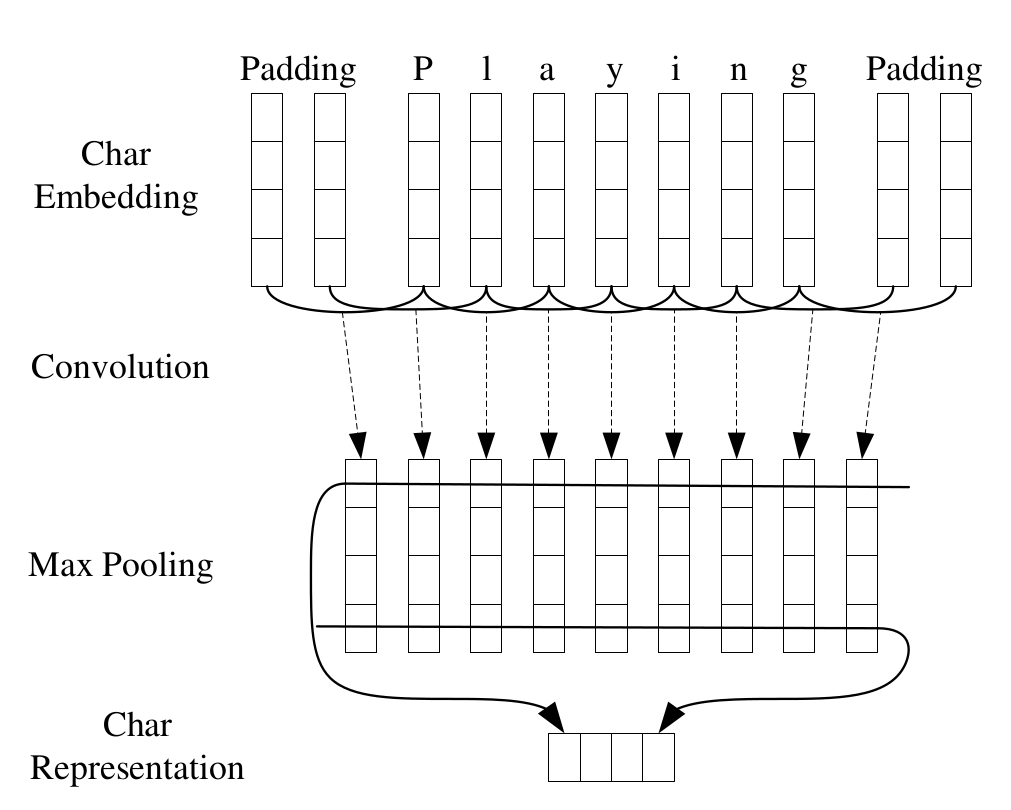
\includegraphics[width=0.4\textwidth]{imgs/cnn_embed.png}
\end{figure}

One dimensional convolution is applied after the dropout which yields character feature vectors. Generated vectors are concatenated with the word embedding vectors. Word embeddings are pretrained vectors that model the inter word relatedness. We used twitter Glove embeddings with vector size of 100.

\section{Dataset}
In this paper, we trained and evaluated models on the dataset that was created from tweets of viewers who watched TV show @midnight. As part of this "game-show" viewers were asked to write a humorous message about a topic that was announced in the show. The day of the ensuing episode, @midnight would create a post that announced the top-10 tweets from the previous episode. The whole dataset consists of 9,658 tweets about 86 different topics. Every tweet in the dataset is labeled in one of the three labels. Label 2 indicates winning tweet, label 1 indicates that tweet was selected as top-10 and label 0 intended for all other tweets. A number of tweets per topic vary among different topics, but 71\% of topics contain at least 90 tweets. Topics with the lowest number of tweets have 20 tweets, and topics with the highest number of tweets have 180 tweets. It is also important to note that for some topics like "FastFoodBooks" external knowledge is required to understand the humor, while for other like "IfIWerePresident" it isn't.

\section{Experiments}

\subsection{Figures}

Here is an example on how to include figures in the paper. Figures are included in \LaTeX{} code immediately \textit{after} the text in which these figures are referenced. Allow \LaTeX{} to place the figure where it believes is best (usually on top of the page of at the position where you would not place the figure). Figures are referenced as follows: ``Figure~\ref{fig:figure1} shows \dots''. Use tilde (\verb.~.) to prevent separation between the word ``Figure'' and its enumeration. 

\subsection{Tables}

There are two types of tables: narrow tables that fit into one column and a wide table that spreads over both columns.

\subsubsection{Narrow tables}

Table~\ref{tab:narrow-table} is an example of a narrow table. Do not use vertical lines in tables -- vertical tables have no effect and they make tables visually less attractive.

\begin{table}
\caption{This is the caption of the table. Table captions should be placed \textit{above} the table.}
\label{tab:narrow-table}
\begin{center}
\begin{tabular}{ll}
\toprule
Heading1 & Heading2 \\
\midrule
One & First row text \\
Two   & Second row text \\
Three   & Third row text \\
      & Fourth row text \\
\bottomrule
\end{tabular}
\end{center}
\end{table}

\subsection{Wide tables}

Table~\ref{tab:wide-table} is an example of a wide table that spreads across both columns. The same can be done for wide figures that should spread across the whole width of the page. 

\begin{table*}
\caption{Wide-table caption}
\label{tab:wide-table}
\begin{center}
\begin{tabular}{llr}
\toprule
Heading1 & Heading2 & Heading3\\
\midrule
A & A very long text, longer that the width of a single column & $128$\\
B & A very long text, longer that the width of a single column & $3123$\\
C & A very long text, longer that the width of a single column & $-32$\\
\bottomrule
\end{tabular}
\end{center}
\end{table*}

Math expressions and formulas that appear within the sentence should be written inside the so-called \emph{inline} math environment: $2+3$, $\sqrt{16}$, $h(x)=\mathbf{1}(\theta_1 x_1 + \theta_0>0)$. Larger expressions and formulas (e.g., equations) should be written in the so-called \emph{displayed} math environment:

\[
b^{(i)}_k = \begin{cases}
1 & \text{if 
    $k = \text{argmin}_j \| \mathbf{x}^{(i)} - \mathbf{\mu}_j \|$}\\
0 & \text{otherwise}
\end{cases}
\]

Math expressions which you reference in the text should be written inside the \textit{equation} environment:

\begin{equation}\label{eq:kmeans-error}
J = \sum_{i=1}^N \sum_{k=1}^K 
b^{(i)}_k \| \mathbf{x}^{(i)} - \mathbf{\mu}_k \|^2
\end{equation}

Now you can reference equation \eqref{eq:kmeans-error}. If the paragraph continues right after the formula

\begin{equation}
f(x) = x^2 + \varepsilon
\end{equation}

\noindent like this one does, use the command \emph{noindent} after the equation to remove the indentation of the row. 

Multi-letter words in the math environment should be written inside the command \emph{mathit}, otherwise \LaTeX{} will insert spacing between the letters to denote the multiplication of values denoted by symbols. For example, compare
$\mathit{Consistent}(h,\mathcal{D})$ and\\
$Consistent(h,\mathcal{D})$.

If you need a math symbol, but you don't know the corresponding \LaTeX{} command that generates it, try
\emph{Detexify}.\footnote{\texttt{http://detexify.kirelabs.org/}}

\section{Conclusion}

We proposed three different models for solving comparative humor ranking task: pairwise comparison task and direct ranking classification task. All three models use deep learning architecture combining approaches of recurrent and convolutional neural networks.

For pairwise comparison task best results were achieved using MODELMODELNAME and were XX\% on development set and YY\% on unseen evaluation data, and for direct ranking classification task best results were achieved using MODELMODELNAME and were XX\% on development set and YY\% on unseen evaluation data. Model evaluation on final unseen data is done using official evaluation scripts given in SemEval-2017 Task 6.

We have compared our results with the results of other task participants resulting in our model ranking  X. out of Y on the Task A, and Z out of K on the Task B.  The main distinction between our model and competitive models is in the lack of hand engineered features which indicates that automatic feature extraction using deep learning framework has a great prospect in this task and requires further work.

For the next step we would experiment with specially adapted word embeddings trained only on the humor containing corpus. We believe it is crucial for word vectors to learn semantic meaning from the domain specific data because of the complex humor structure.  TODO: One short sentence about number of parameters and overfitting.

\section*{Acknowledgements}

Hvala svima u studiju i režiji.

\bibliographystyle{tar2016}
\bibliography{tar2016} 

\end{document}

